\documentclass[12pt,a4paper]{article}
\usepackage{amsmath,amssymb,graphicx}
\usepackage{bbm}
\usepackage{authblk}
\usepackage{faktor}
\usepackage{caption}
\usepackage{subcaption}
\usepackage{float}
% \usepackage{tcolorbox}
\usepackage[utf8]{inputenc}
\usepackage[english]{babel}
\usepackage{listings}
\usepackage{color}


\begin{document}

\title{ Notes on Simple Nets }

\author[$\dagger$]{}
%\affil[$\dagger$]{Department of Theoretical Physics, Maynooth University}
\date{}

\maketitle


\section{Overall plan}

(v.1: Masud, August 2019)

The current idea of the project:

\begin{center}\emph{Fitness landscape of 3-node and 4-node neural networks}
\end{center}

Restricting to one input node and one output node, we can think of three network geometries:

\begin{center}
\begin{tabular}{l|l}
\hline
%
\parbox{0.42\textwidth}{ 
%

\begin{center}\includegraphics[width=0.4\textwidth]{Images/3_architectures_a_01}
\end{center}


} &   \hspace{-0.01\textwidth}
\parbox{0.48\textwidth}{ \flushleft

\begin{itemize}

\item[(A)] One hidden layer, containing a single hidden node. \\ 4 parameters. 

\bigskip 

\item[(B)] Two hidden layers, each containing a single node. 
  \\ 6 parameters.
  
\bigskip 

\item[(C)] One hidden layer, consisting of two nodes. 
  \\ 7 parameters.
  
\end{itemize}

} 
\\
\hline
\end{tabular}
\end{center}



We can then explore and describe the landscape of the loss function for the same (or similar)
learning task in these three cases.  In addition, we can explore and describe how the gradient descent moves us along
this landscape.

The three networks have respectively 4, 6 and 7 parameters.

The primary learning task with these networks will be to learn a scalar function.  The function
$f(x) = x^2$ seems the most natural to concentrate on.  We still have to specify the domain of the
function (interval from which $x$ is chosen) over which to concentrate on.  We might want to use the
sigmoid function in the definition of the network; in that case the outputs are limited to $[0,1]$.
Hence it makes sense to use the interval $[-1,1]$.

The 3-node network (A) is so limited that it is not able to approximate the parabolic shape in the
whole range $[-1,1]$ (please double-check this statement), so we will probably have to limit it to
$[0,1]$.

The choice of activation function defines the network, i.e., the loss function will depend on the
activation function.  Let's start with the sigmoid whenever we can, and possibly play with using
other activation functions later.



\newpage 


\section{The 3-node network}

(v.1: Masud, August 2019)

The function represented by the network is
\begin{equation}
N(x) ~=~  \sigma\Big( w_2 \sigma\big(w_1x+b_1\big) +b_2 \Big)
\end{equation}
So the quantity we want to analyze is
\begin{equation}
L(w_1,w_2,b_1,b_2) ~=~  \int_{x_{\rm min}}^{x_{\rm max}} \Big[ N(x) -x^2 \Big]^2 
\end{equation}
In practice we want to discretize this integral and have a sum over a grid of $x$ values.  Hopefully
the answer does not depend much on the discretization.  



\newpage

\section{The diamond network}

(v.1: John, August 2019)

\subsection{Introduction}

We trained a simple neural net to learn the function $f(x)=x^2$ and explore aspects of the landscape of the related loss function. The network we trained, depicted in Fig.\ref{DiamondNet}, has a single input neuron, a single hidden layer with two neurons and a single output neuron. The network we trained uses the sigmoid function as its activation function and so the output of the network is a number in the interval $[0,1]$. For this reason, we focus on learning the function $f(x)=x^2$ over the domain $[-1,1]$ so that the range of $f$ matches the range of out network.

\begin{figure}
\center
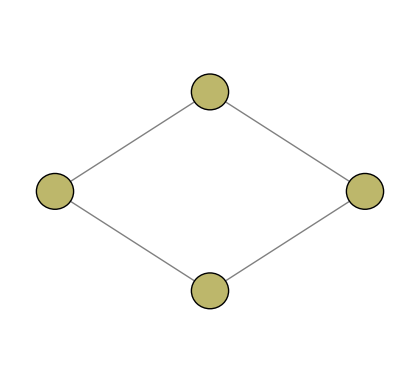
\includegraphics[scale=0.5]{Images/net_1_2_1.png}
\caption{}
\label{DiamondNet}
\end{figure}


To train the network, we generated an array of random 10000 points uniformly distributed in the interval $[0,1]$ and then computed the value of $f(x)$ for each random point. This gave us a data set to train our network on. A second data set was generated, in the same way, to be used for testing how well the network generalises. The network was trained using the stochastic gradient decent method for 50 epochs with a mini-batch size of 50. The evolution of the networks output as function of $x$ is shown in Fig.\ref{training}

\begin{figure}
\begin{subfigure}{.32\textwidth}
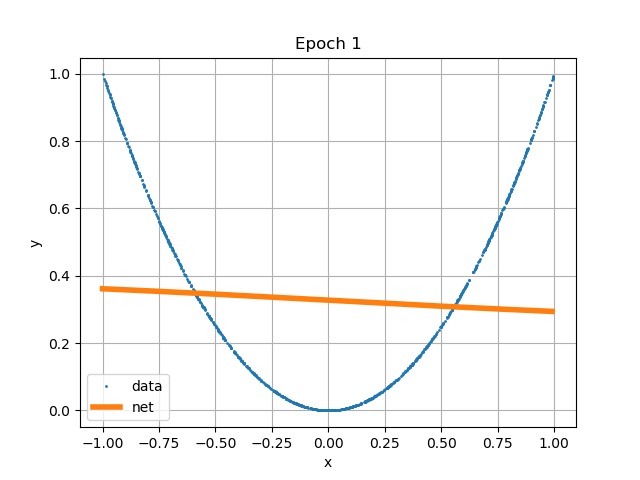
\includegraphics[scale=0.3]{Images/ALearningNet1.png}
\caption{}
\label{training1}
\end{subfigure}
\begin{subfigure}{.32\textwidth}
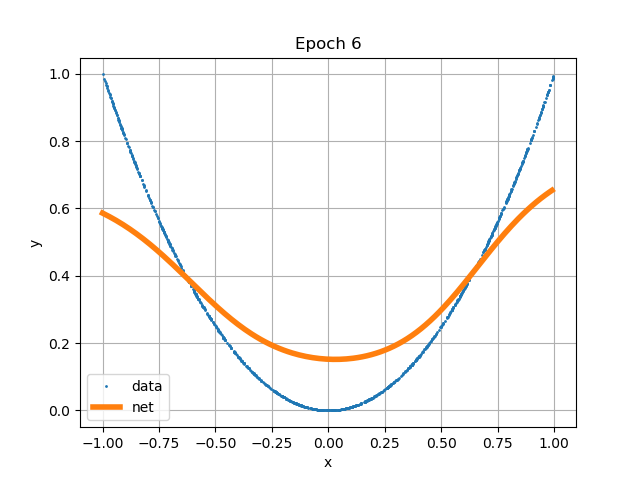
\includegraphics[scale=0.3]{Images/ALearningNet6.png}
\caption{}
\label{training2}
\end{subfigure}
\begin{subfigure}{.32\textwidth}
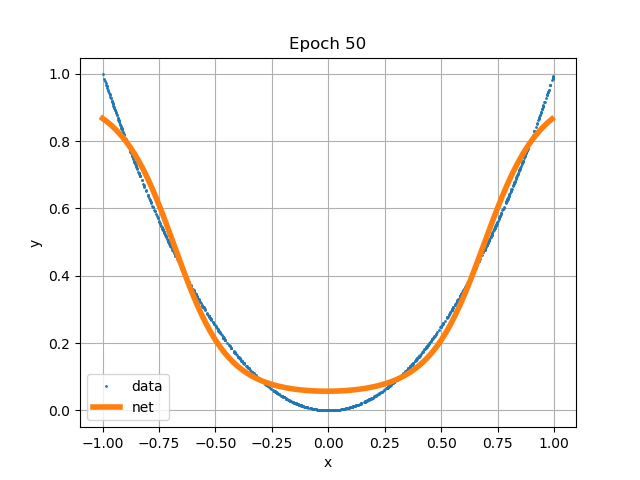
\includegraphics[scale=0.3]{Images/ALearningNet50.png}
\caption{}
\label{training3}
\end{subfigure}
\caption{}
\label{training}
\end{figure}

Once the network had been trained, we then looked at the performance of the network. The loss function used to evaluate the performance of the net was the squared Euclidean distance between the output of the net and the target output averaged over the test data.

The change in loss due to a variation in each of the networks parameters was calculated. We number the parameters of the network 0 to 6. The weights connecting the first two layers are numbers 0 and 1 while the weights connecting the second and third layers are numbered 2 and 3. The biases of the hidden layers are numbered 4 and 5 while the bias for the output neuron is given the number 6. Given the trained weights and biases $\{\omega_i\}$, we vary a particular parameter by adding a constant $\delta \omega_i$ ranging from -10 to 10 while holding all other parameters fixed. The results are shown in Fig.\ref{LossNearTrainedWeights}. We see each curve having a local minimum at $\delta\omega_i = 0$ indicating the network found a local minimum of the loss function while being trained.

\begin{figure}[H]
\center
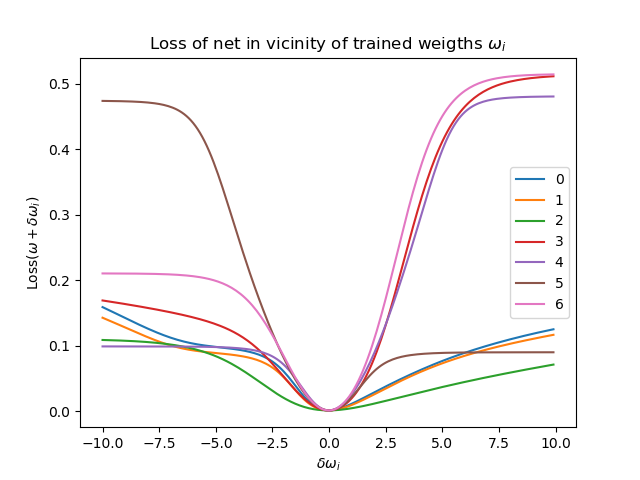
\includegraphics[scale=0.5]{Images/LossInVicinityOfTrainedWeights.png}
\caption{}
\label{LossNearTrainedWeights}
\end{figure}



\end{document}
